
\begin{frame}{Super-Resolution Imaging}
    \begin{block}{Cos'è la Super-Resolution Imaging?}

        \begin{itemize}
            \item È una tecnica di machine learning
            \item Migliora la definizione di un immagine a bassa risoluzione
            \item Trova applicazioni nei seguenti campi:
            \begin{itemize}
                \item Immagini mediche (Risonanze, TAC)
                \item Upscaling di immagini o video
            \end{itemize}
        \end{itemize}

    \end{block}

    \vspace{0.3cm}


\end{frame}

\begin{frame}{Pipeline di super-resolution}
    \centering

  % Nel preambolo: \usepackage{tikz}
  %                \usetikzlibrary{arrows.meta, positioning}
  \begin{tikzpicture}[
      node distance = 0.45cm,
      box/.style = {
        rounded corners=3pt,
        minimum width=4cm,
        minimum height=0.7cm,
        align=center,
        font=\small\bfseries,
        text=white
      },
      arr/.style = {-{Stealth[length=5pt]}, thick, gray}
    ]

    \node[box, fill=red!70!black] (lr)
      {Immagine LR\\[1pt]
       {\footnotesize\normalfont bassa risoluzione}};

    \node[box, fill=blue!40!black, below=of lr] (up)
      {Upsampling bicubico\\[1pt]
       {\footnotesize\normalfont pre-processing}};

    \node[box, fill=teal!60!black, below=of up] (cnn)
      {Rete CNN\\[1pt]
       {\footnotesize\normalfont apprendimento dettagli}};

    \node[box, fill=green!40!black, below=of cnn] (sr)
      {Immagine SR\\[1pt]
       {\footnotesize\normalfont alta risoluzione}};

    \draw[arr] (lr)  -- (up);
    \draw[arr] (up)  -- (cnn);
    \draw[arr] (cnn) -- (sr);

  \end{tikzpicture}
\end{frame}

\begin{frame}{Architettura rete}

    \begin{block}{Rete CNN}

     \begin{itemize}
        \item Rete CNN come approccio classico
        \item Ispirato al paper: \textbf{\quotes{Deep Learning (SRCNN, 2014)}}
        \item Tre layer di convoluzione, 64 canali in output dal primo layer
        \item Prende in input il canale della luminanza
    \end{itemize}

    \end{block}

    {\centering
    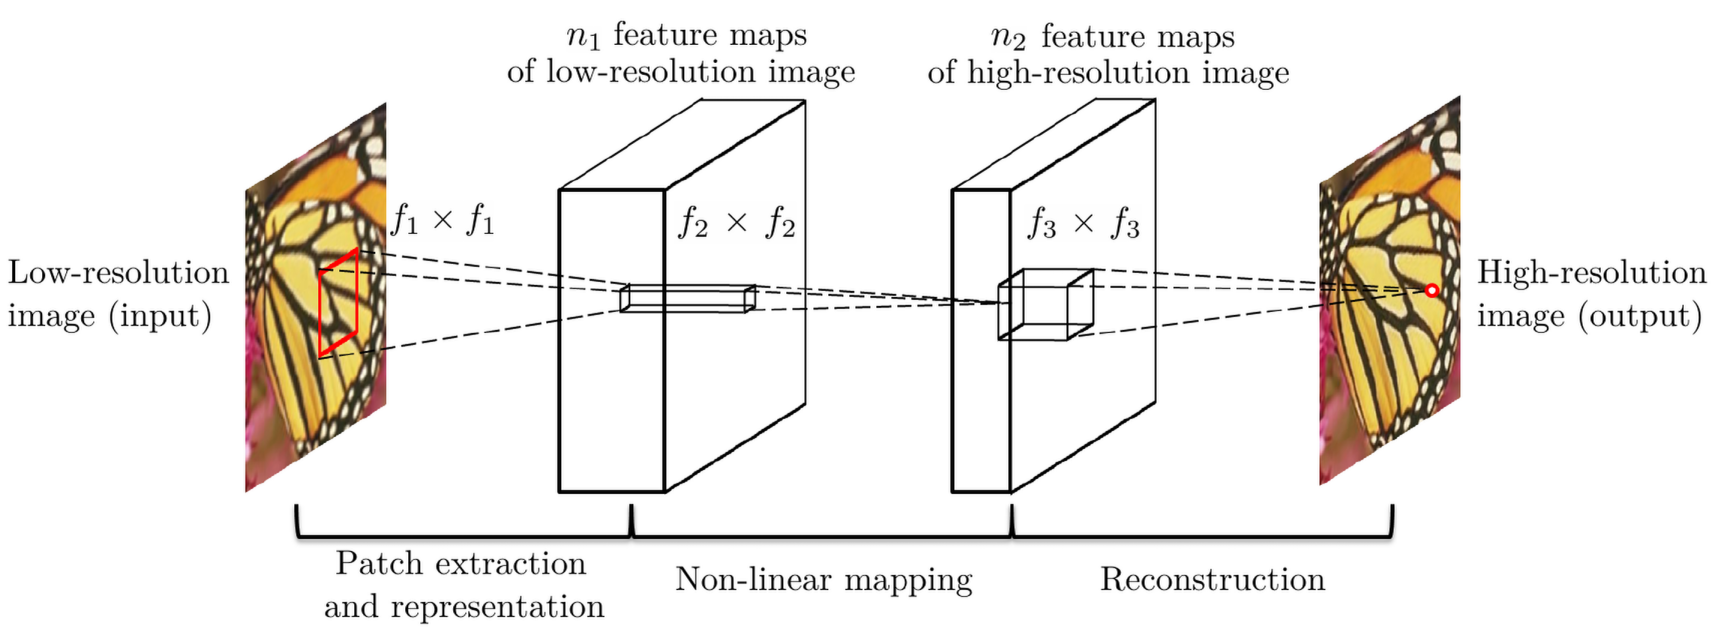
\includegraphics[width=0.8\textwidth]{figures/architettura_SRCNN.png}
    \par}
\end{frame}

\begin{frame}{Obiettivo e Metrica di Valutazione}

    \begin{block}{Obiettivo}
        Superare le prestazioni dell'interpolazione bicubica nella di ricostruzione/super-resolution delle immagini.
    \end{block}
    \vspace{0.5cm}
    \begin{block}{Metrica di Validazione}
        Utilizzo del \textbf{PSNR} (\textit{Peak Signal-to-Noise Ratio}) per valutare quantitativamente la fedeltà del segnale visivo rispetto all'immagine originale.
    \end{block}

\end{frame}

\begin{frame}{Pipeline di training e validazione}
    \centering
% Nel preambolo: \usepackage{tikz}
%                \usetikzlibrary{arrows.meta, positioning}
\resizebox{\textwidth}{!}{%
\begin{tikzpicture}[
      node distance = 0.6cm,
      box/.style = {
        rounded corners=3pt,
        minimum width=3.2cm,
        minimum height=1cm,
        align=center,
        font=\small\bfseries,
        text=white
      },
      arr/.style = {-{Stealth[length=5pt]}, thick, gray}
    ]
\node[box, fill=violet!55!black] (patch)
      {Estrazione patch\\[1pt]
       {\footnotesize\normalfont 40 patch 128$\times$128 casuali}};
\node[box, fill=teal!60!black, right=of patch] (train)
      {Training CNN\\[1pt]
       {\footnotesize\normalfont Addestramento sulle patch}};
\node[box, fill=blue!40!black, right=of train] (val)
      {Validazione\\[1pt]
       {\footnotesize\normalfont 200 immagini di validazione}};
\node[box, fill=green!40!black, right=of val] (save)
      {Calcolo PSNR medio\\[1pt]
       {\footnotesize\normalfont Salvataggio best model}};
\draw[arr] (patch) -- (train);
\draw[arr] (train) -- (val);
\draw[arr] (val)   -- (save);
\end{tikzpicture}%
}

\vspace{1cm}

\begin{block}{Dataset utilizzati}
    \begin{itemize}
        \item DIV2K: immagini ad alta risoluzione; usato per training e validation:
        \begin{itemize}
            \item 800 per training, vengono estratte 40 patch da 128x128 per ogni immagine
            \item 200 per validation
        \end{itemize}
        \item SET5: 5 immagini a bassa risoluzione usate per il test set
        \item La fase di validazione è fatta dopo ogni epoca di training
        \item Come loss function è stata usata la MSE
    \end{itemize}
\end{block}

\end{frame}

\begin{frame}{Risultato migliore rete paper 2014}
    \begin{block}{Risultati}
        \begin{itemize}
        \item Non è stata superata nessuna istanza del test set.
        \item Nel miglior risultato la rete CNN è indietro di 3 unità rispetto all'interpolazione bicubica
        \item Risultati dovuti probabilmente a pochi layer di convulizione e anche un dataset diverso da quello del paper
    \end{itemize}

    \end{block}

    {\centering
    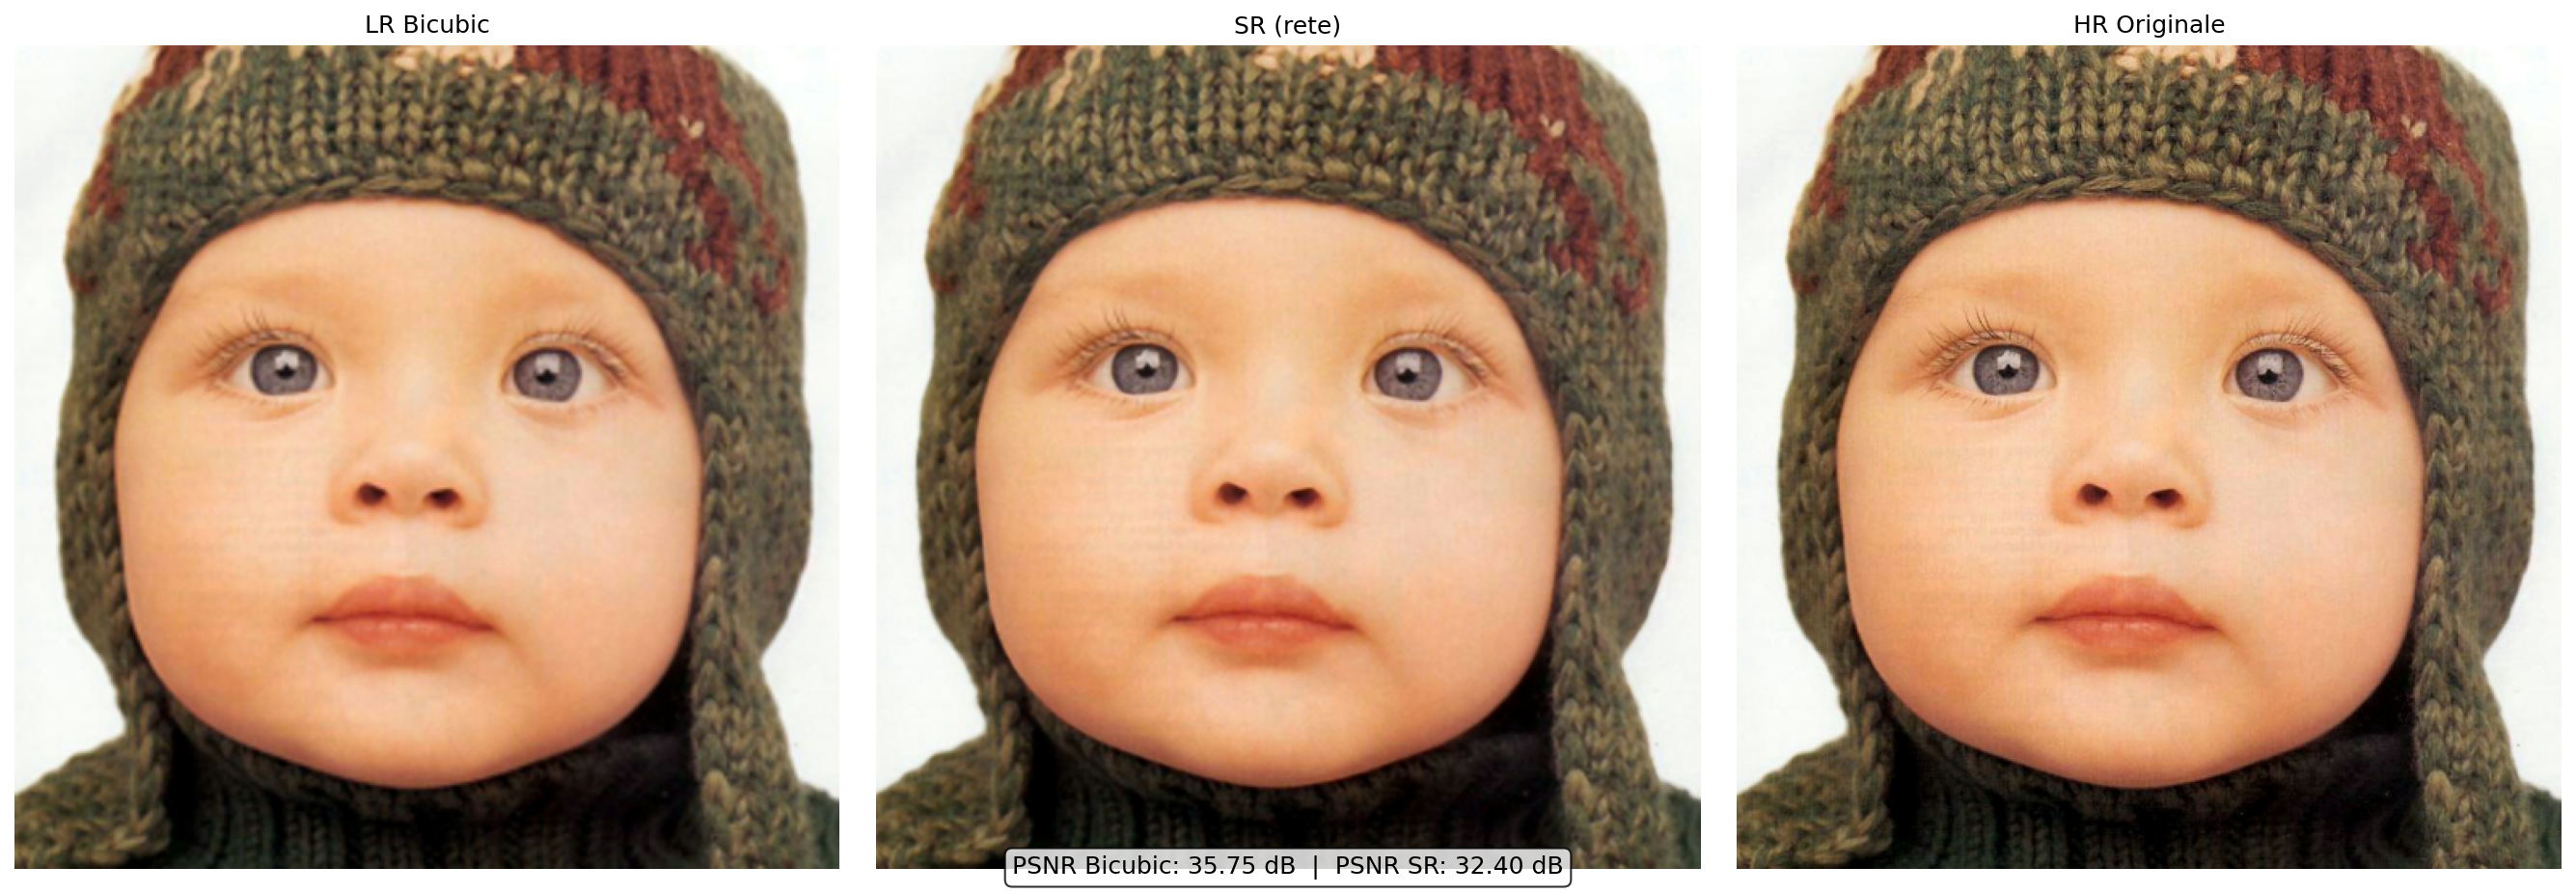
\includegraphics[width=0.8\textwidth]{figures/confronto_srcnn(9-5-5)_model_600_epochs_2026-05-23_13-06-36 copy.png}
    \par}
\end{frame}
